\section{Experiments}
\label{sec:experiments}

In this section, we describe the empirical study of our \trip solver for the itinerary planning problem.

\subsection{Dataset Description}
\label{sec:dataset}

In order to test our itinerary planning system, we used curated datasets of Points of Interest (POIs) for six large cities: Budapest, Delhi, Edinburgh, Glasgow, Osaka, and Vienna. 
%\ari{Americans will be very unhappy.} \ab{Ha ha ha!}
The dataset utilized for our work is derived from the \emph{Yahoo Flickr Creative Commons 100 Million Dataset (YFCC100M)}~\cite{taylor2018tour} containing over 100 million images, of which 69 million are annotated and 48 million are geotagged.
%
The authors of~\cite{taylor2018tour} considered a set of popular POIs for the cities mentioned earlier using resources such as \emph{Wikipedia}. Then, geotagged photos in \emph{Flickr} were matched with these POIs using spatial proximity. The relative popularity of a POI, used as the measure for its \textbf{utility}, was estimated based on the number of photos associated with each POI. The Flickr User-POI Visits dataset, curated in this manner by~\cite{limkwanhuiDataCode}, is used in our work.
This provides a practical way to understand how tourists behave by using publicly shared photos as a proxy for how much interest people have in a particular place.

Table~\ref{tab:original} contains the original dataset fields. With an aim to make our system more realistic and practical to use, we augmented the fields by adding some more features, as listed in Table~\ref{tab:additional}.
These additional information were collected by either scraping or quoting official tourist boards, city tourism websites, and trustworthy travel websites.

\begin{table}[t]
\begin{tabular}{l l}%p{4cm}}
\toprule
\textbf{Field Name} & \textbf{Description} \\
\midrule
\texttt{ID} & Unique ID of the POI\\%assigned to each POI. \\
%\hline
\texttt{Name} & Name of the POI\\%, e.g., ``Red Fort'', ``Osaka Castle''. \\
%\hline
\texttt{Location} & Location of the POI in terms of latitude and longitude \\
%\texttt{Latitude} & Latitude\\%coordinate of the POI. \\
%\hline
%\texttt{Longitude} & Longitude\\%coordinate of the POI. \\
%\hline
\texttt{Category} & Theme or Type of the POI\\% classification of the POI, such as \textit{amusement}, \textit{historical}, \textit{museum}, \textit{shopping}, \textit{park}, etc. \\
%\hline
\texttt{Utility} & Numerical value representing estimated utility of the POI\\% or attractiveness of the POI, derived based on its popularity (photo frequency). \\
%\hline
\texttt{Distance} & Distance to other POIs\\%. This is used in the travel time estimation between locations, with the walking speed $v_w$ and taxi speed $v_t$. \\
\bottomrule
\end{tabular}
\tabcaption{Original dataset fields}
\label{tab:original}
\end{table}

\begin{table}[t]
\centering
\begin{tabular}{l l}
\toprule
\textbf{Field Name} & \textbf{Description} \\
\midrule
\texttt{Visit Cost} & Visit cost of the POI including entrance fee, etc.\\%Entrance fee or ticket price associated with the POI, in INR. \\
%\midrule
\texttt{Visit Time} & Average time spent by tourists in the POI\\%duration (in minutes) tourists typically spend at the POI. \\
%\midrule
\texttt{Opening Time} & Time of the day when the POI opens\\%The time at which the POI opens for visitors, stored in \texttt{HH:MM:SS} format. \\
%\midrule
\texttt{Closing Time} & Time of the day when the POI closes\\%The time at which the POI closes for visitors, stored similarly. \\
%\midrule
\texttt{Days of Week} & Days when the POI is open\\%Seven binary columns (\texttt{Monday}, \texttt{Tuesday}, ..., \texttt{Sunday}). A value of 1 indicates the POI is open on that day; 0 indicates it is closed. \\
\texttt{Travel Time} & Travel time to other POIs for each mode of transport \\
\texttt{Travel Cost} & Travel cost to other POIs for each mode of transport \\
\bottomrule
\end{tabular}
\tabcaption{Additional features added to the dataset}
\label{tab:additional}
\end{table}

\subsection{Configuration}

The experiments were conducted on a high-performance Linux server equipped with dual Intel(R) Xeon(R) E5-2697 v3 CPUs, each running at 2.60\,GHz, providing a total of 56 logical processors (28 physical cores per socket with hyper-threading enabled) and 503\,GB of RAM.
The code was implemented in Python and mixed integer linear programming was done in Gurobi.

\subsection{Baseline Itinerary Planner}

To evaluate the performance of the \trip solution, we identified the works \cite{bolzoni2014efficient,taylor2018tour} and \cite{chen2014automatic,vanzelst2016itinerary} as potential baselines for single day itinerary planning and multi-day itinerary planning, respectively. This choice was based on the features of the solutions, as listed in Table~\ref{tab:otherworks}. Although we requested the authors of the respective works to share their implementation codes we did not receive a suitable response. Moreover, while the works \cite{bolzoni2014efficient,taylor2018tour}  consider utility optimization as their objective, the works \cite{chen2014automatic,vanzelst2016itinerary} did not. In addition, the implementation details stated in \cite{bolzoni2014efficient} were insufficient to reproduce their solution.  We, thus, did a best-effort implementation of~\cite{taylor2018tour}. While it too lacked a code repository or implementation details like the POI visiting durations, we were able to at least replicate the key features and constraints described. 
Hence, we consider \cite{taylor2018tour} to be the  \emph{baseline} for evaluating single day as well as multi-day itinerary planning.

Despite our best efforts, a direct performance comparison between our model and the baseline may not be
feasible due to a key limitation in the common dataset used by both our
system and~\cite{taylor2018tour}.
This pertains to the POI visit time field.
Since the code and dataset of~\cite{taylor2018tour} is not available, we are not sure what values they used for POI visit times.
Nevertheless, we assume that they will not be very different from the average values used by us.
Another limitation of the algorithm of~\cite{taylor2018tour} was that it did not consider any cost budget during
itinerary planning.
Thus, to ensure a fair comparison with their approach, we used a very
high cost budget in our experiments when compared with the baseline, so that
it would not influence the itinerary planning outcome.

\subsection{Variants of \trip}

We evaluate the performance of the \trip solution by considering all the utility variants (binary, slab, continuous) as well as the transportation mode variants (walking, taxi, hybrid). We, thus, have a total of $3 \times 3 = 9$ \trip variants.

\subsection{Performance Metrics}

We evaluate the performance of the baseline and the \trip variants on mainly \emph{utility}, since that is what the objective of the optimization function is.
In addition, however, we also measure the following parameters:

\begin{enumerate}
    \item \emph{Running time} of the solver, to determine its practicality
    \item \emph{Time and Cost spent} as a ratio of the total time and cost budget, to understand the utilization efficiency
    \item \emph{Time and Cost profile} of how time and cost are spent for travel vis-a-vis POI visit
\end{enumerate}

\begin{figure}[t]
\centering
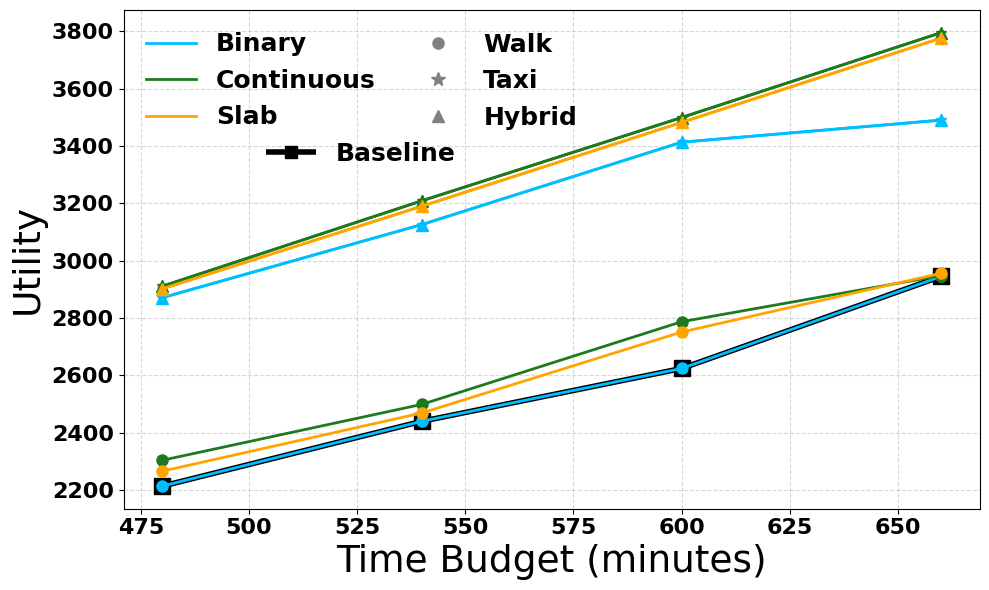
\includegraphics[width=\figwidth]{plots/baseline_singleDay.png}
\figcaption{Comparison of \trip variants with baseline}
\label{fig:baseline-single}
\end{figure}

\subsection{Comparison with Baseline}

We first experiment to see the performance of \trip against the baseline.
Fig.~\ref{fig:baseline-single}\footnote{This and all subsequent graphs use a combination of line colors for utility variants and point shapes for transportation modes. Since there are 3 utility variants and 3 transportation modes, a combination of these legends produces the 9 \trip variants. For example, since Binary is represented by cyan-colored lines and Walking by circles, a cyan-colored line with circles represent the Binary Walking variant of \trip.}
shows the utility scores across different time budgets under a high cost budget scenario (100000 units) for the city of Osaka for a single day.
As expected, utility increases with increasing time budget, since there is more time to visit more POIs.
Notably, the \trip Binary-Walking variant closely replicates the behavior of the baseline model, validating its correctness and fairness for comparative purposes. The other models, especially the Hybrid mode ones, outperform the baseline significantly.
Since the cost budget is very high, the utility scores of Taxi match those of Hybrid.

%Overall, the plot effectively highlights how our approach—especially the allowance for partial POI visits and the use of flexible transport—leads to significantly improved itinerary recommendations, both in terms of utility and adaptability to real-world constraints.

\begin{figure}[t]
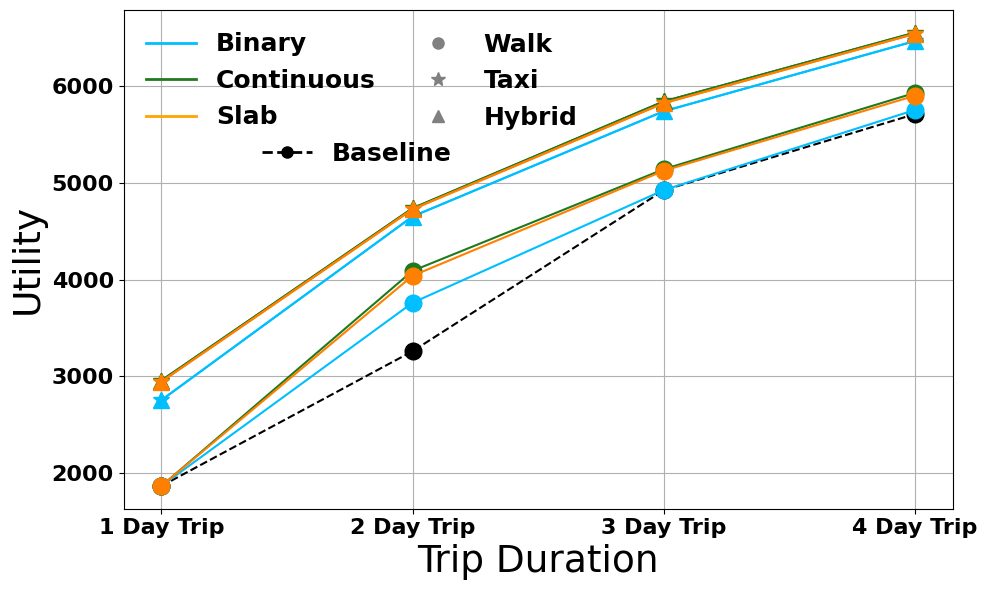
\includegraphics[width=\figwidth]{plots/baseline_multiDay.png}
\figcaption{Comparison against baseline for multi-day trips}
\label{fig:baseline-multi}
\end{figure}

We next experiment with multi-day itinerary on Osaka for a very high cost budget of 100000 to ensure that cost is not a limiting factor for the baseline.
Each day was assigned a time budget of 8 hours.
Fig.~\ref{fig:baseline-multi} shows the results for 1 to 4 days.
The baseline utilities were calculated by creating daily itineraries one after another, making sure not to repeat any POIs from previous days, and summing up the utilities.
The \trip variants run optimized multi-day planning models and, consequently, perform much better. Given the consistent and significant advantage of \trip over the baseline, we chose to leave the baseline out of future comparisons.

\begin{figure*}[t]
	\centering
    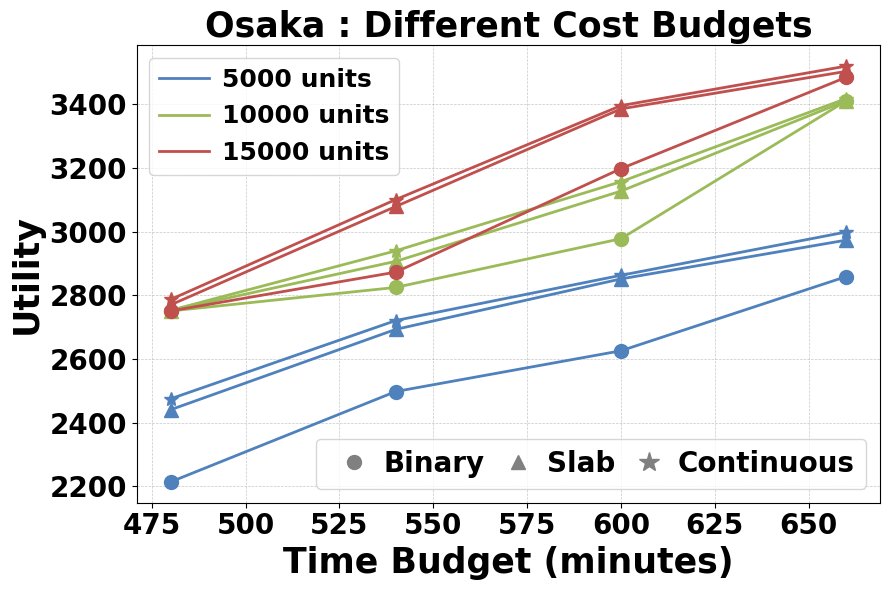
\includegraphics[width=0.60\columnwidth]{plots/exp1-osaka.png}
    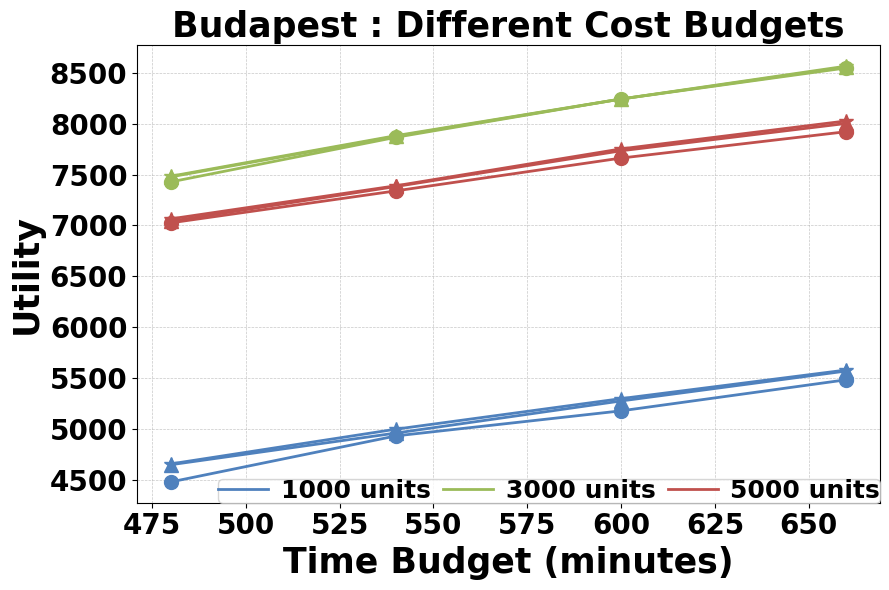
\includegraphics[width=0.60\columnwidth]{plots/exp1-budapest.png}
    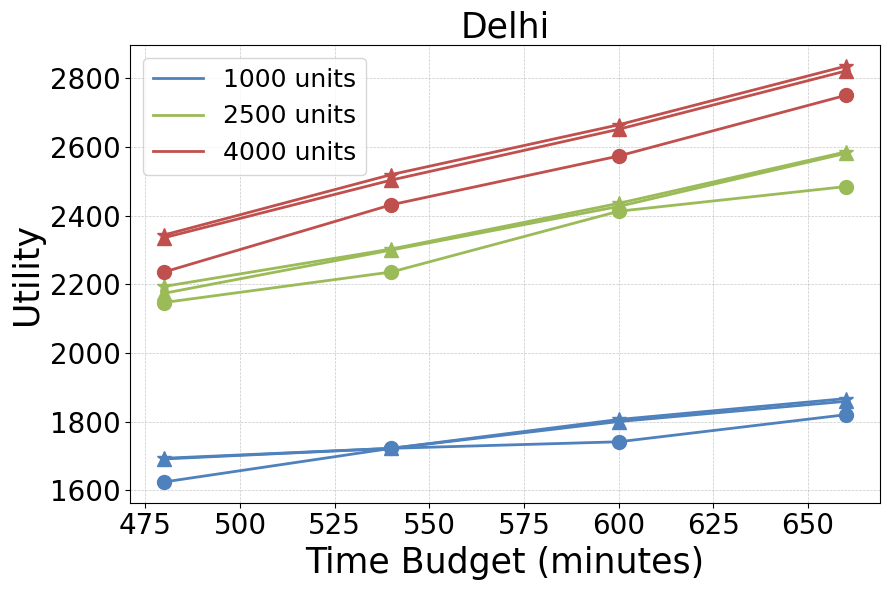
\includegraphics[width=0.60\columnwidth]{plots/exp1-delhi.png}
    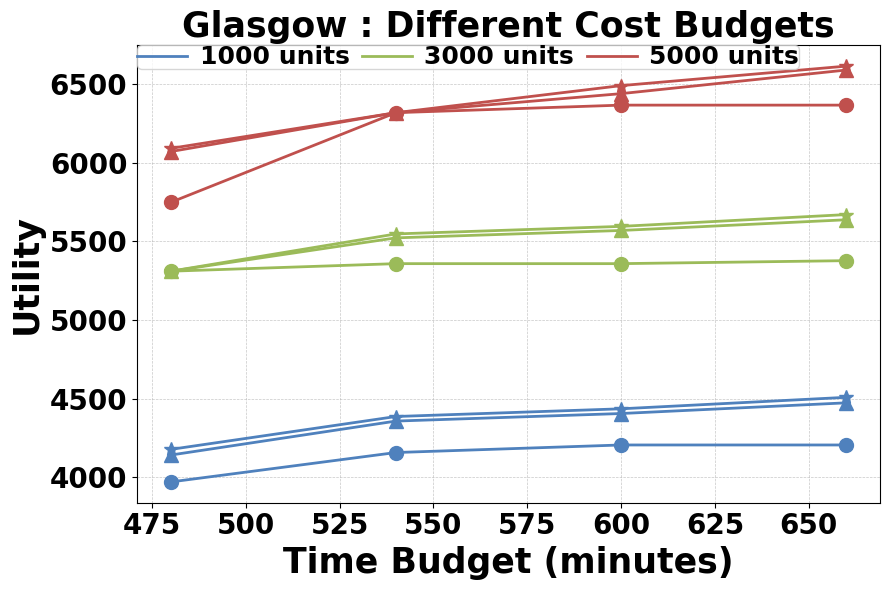
\includegraphics[width=0.60\columnwidth]{plots/exp1-glasgow.png}
    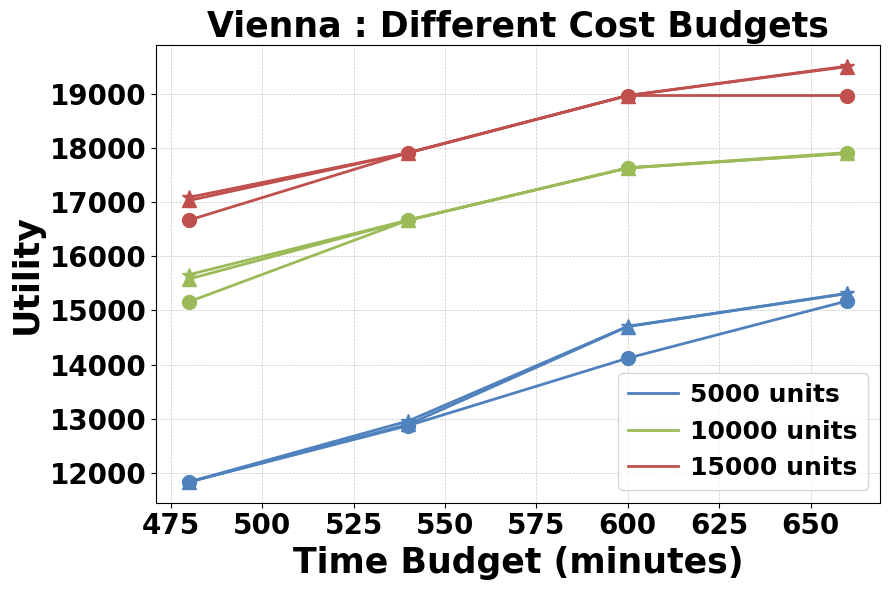
\includegraphics[width=0.60\columnwidth]{plots/exp1-vienna.png}
    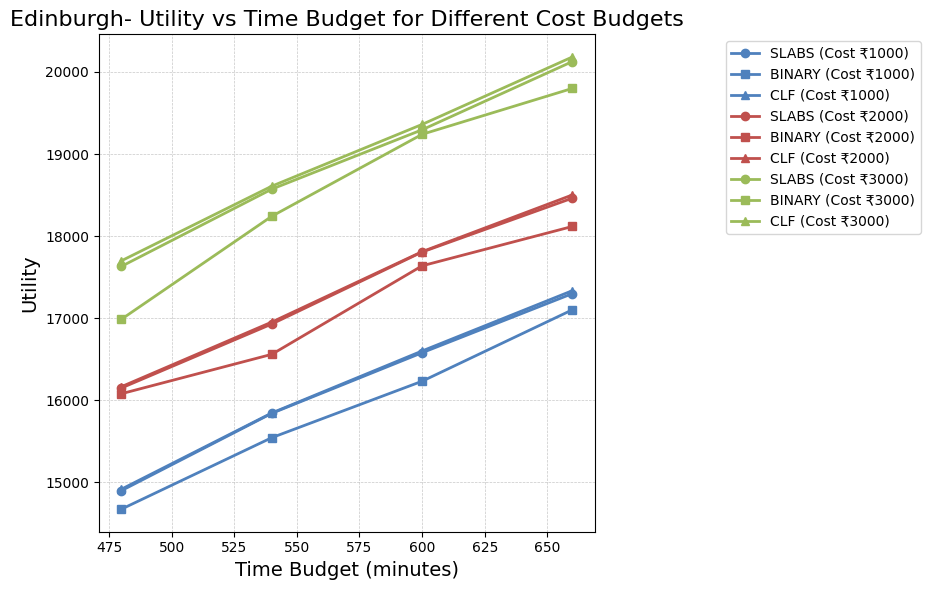
\includegraphics[width=0.60\columnwidth]{plots/exp1-edinburgh.png}
    \figcaption{Utility variation with different time and cost budgets for 6 cities}
    \label{fig:cities}
\end{figure*}

\subsection{Multiple Cities}

Fig.~\ref{fig:cities} shows the results of single day tour planning for 6 different cities under various time and cost budgets for different utility variants for the Hybrid mode.
The time budget is varied within a practical range of 480 to 600 minutes, and the cost budget is chosen to be appropriately aligned with the economic characteristics of the city.
As expected, higher cost and time budgets allow for higher utilities.
The Continuous utility variant shows the best performance.
%\ab{can we have utilization numbers here?}
Since the trends remain the same across the cities, we choose Osaka as a representative, and show all subsequent results for it only.

\subsection{Effect of Multi-modality}

\begin{figure}[t]
\centering
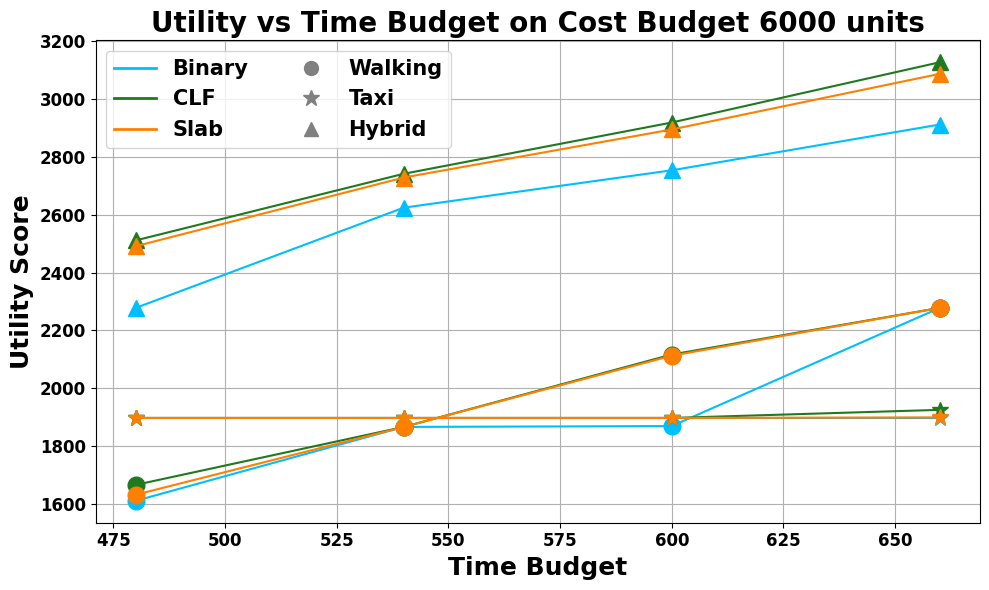
\includegraphics[width=\figwidth]{plots/multimodality1.png} \\
(a) Fixed cost budget of 6000 units 
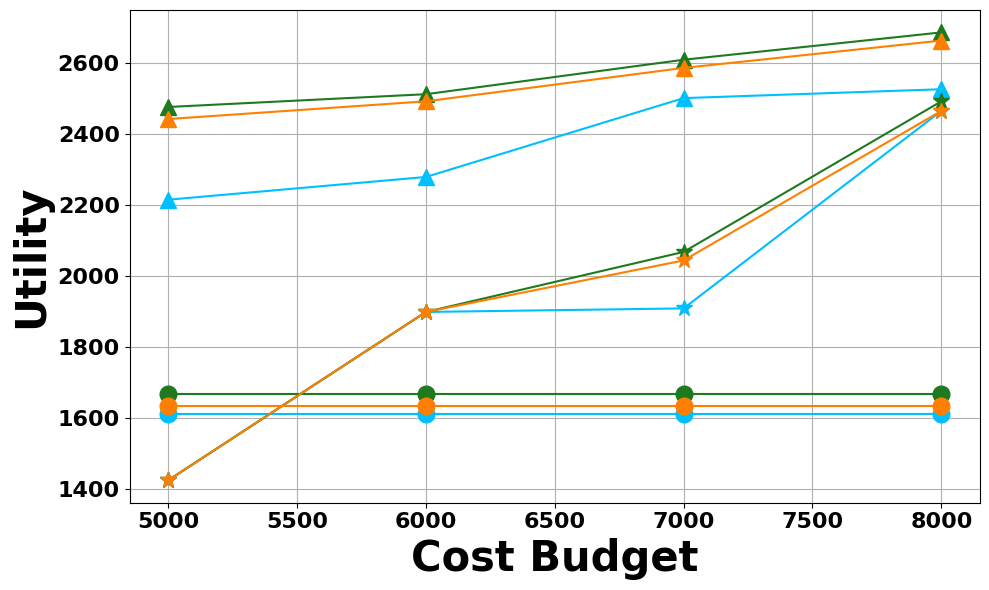
\includegraphics[width=\figwidth]{plots/multimodality2.png} \\
(b) Fixed time budget of 480 minutes
\figcaption{Effect of transportation modes}
\label{fig:multi-modal}
\end{figure}

We next evaluate the effect of multiple modes of transport (Fig.~\ref{fig:multi-modal}).
For a fixed cost budget (of 6000 units), the top graph shows that Hybrid is generally the best mode by a significant margin. This is intuitive since Hybrid chooses the best of both the worlds.
The utility obtained using only Taxi saturates after a while, since once the fixed cost budget is exhausted, it cannot visit any more POI.
The bottom graph shows the effect of increasing cost budget for a fixed time budget of 480 minutes.
Again, while Hybrid is the best mode, with larger cost budgets, the Taxi variant catches up quickly.
This is intuitive since a large cost budget allows the traveler to quickly visit multiple POIs by spending more on taxi.
Since walking does not incur any cost, for a fixed time budget, there is no effect of the cost budget on it, and the utility remains the same.
Among the utility variants, Continuous shows the best performance.

\subsection{Time and Cost Profile}

\begin{figure}[t]
\centering
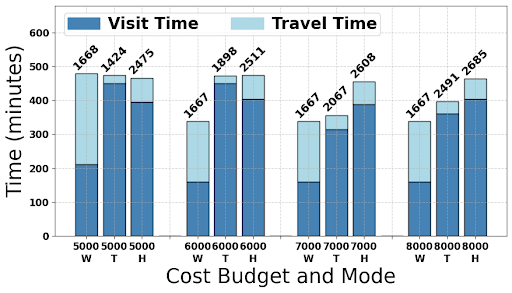
\includegraphics[width=\figwidth]{plots/tu1.png} \\
(a) Fixed time budget of 480 minutes (Continuous)
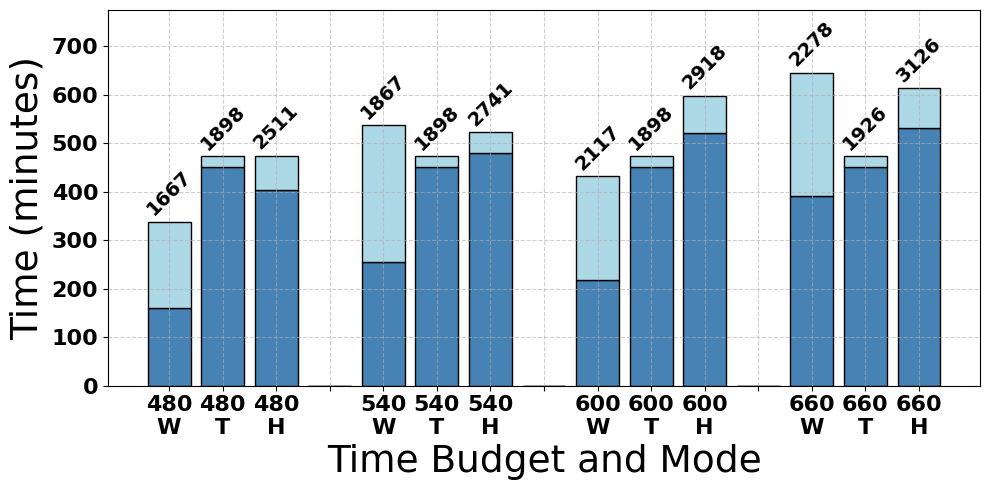
\includegraphics[width=\figwidth]{plots/tu2.png} \\
(b) Fixed cost budget of 6000 units (Continuous)
\figcaption{Time utilization (numbers on bars show utility scores)}
\label{fig:time-utilization}
\end{figure}

To understand the effects of different modes of transport even better, we next plot the time and cost utilization profiles.

Fig.~\ref{fig:time-utilization} shows how the time is spent across visiting POIs versus traveling between POIs for different time and cost budgets.
Walking shows a high travel-to-visit time ratio, which is expected due to the slow nature of walking. A significant amount of time is, thus, spent in traveling. On the other extreme, Taxi minimizes travel time. Hybrid offers a solution which is mid-way, and achieves a more moderate ratio and a better utility.
Across all variants, increasing time budget allowed better utilization of available time, with Hybrid mode consistently providing the most balanced performance. This highlights that optimizing for utility involves not just maximizing visit duration but also strategically balancing travel efficiency with multi-modal flexibility.

Further, the Hybrid mode consistently achieves high time utilization, utilizing more than 95\% of the time budget, across all time and cost budgets. 
The Taxi mode shows better time utilization with smaller time budgets. For a higher time budget, since the cost budget is fixed, it quickly exhausts the cost and, consequently, fails to utilize the rest of the available time.
With increasing cost budget, however, it again improves the time utilization.

\begin{figure}[t]
\centering
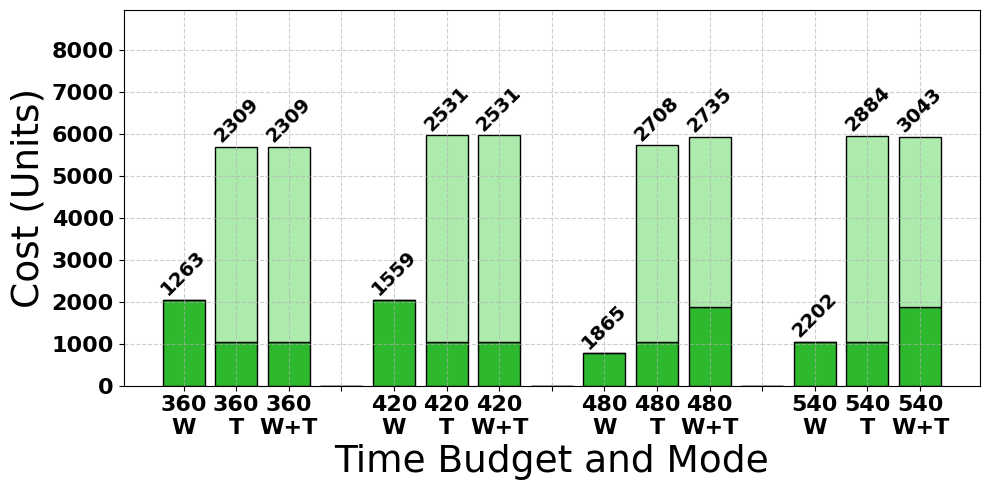
\includegraphics[width=\figwidth]{plots/cu5.png} \\
(a) Fixed time budget of 480 minutes (Continuous)
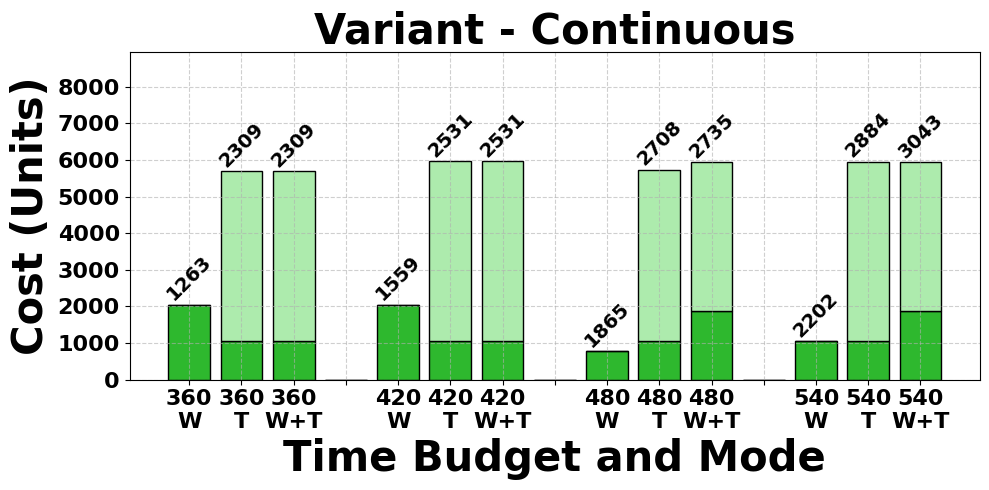
\includegraphics[width=\figwidth]{plots/CU1.png} \\
(b) Fixed cost budget of 6000 units (Continuous)
\figcaption{Cost utilization (numbers on bars show utility scores)}
\label{fig:cost-utilization}
\end{figure}

Fig.~\ref{fig:cost-utilization} shows the corresponding cost utilization profiles for the same experiments.
The POI visit costs are typically lower than the travel costs.
Hybrid offers a better ratio since it can visit more POIs.
Cost utilization, however, is not always an indicator of utility maximization.
The cost of visiting a POI is not always proportional to its utility.
In Taxi mode, although faster travel allows reaching distant POIs, the high travel cost often exhausts the budget before accessing faraway high-utility POIs. Thus, for low cost budgets, its visit utilization is lower and utility is poorer.

\subsection{Multi-day Trips}

\begin{figure}[t]
\centering
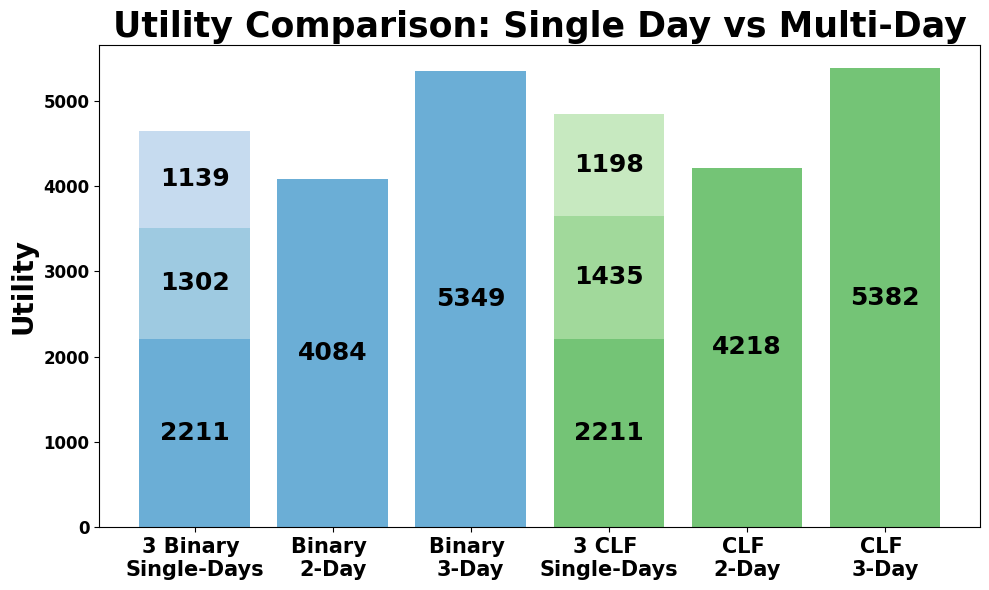
\includegraphics[width=\figwidth]{plots/multivssingle.png}
\figcaption{Benefits of solving a single multi-day optimization problem against aggregating over several single-day itineraries}
\label{fig:multi-day}
\end{figure}

We next measure the effect of optimizing the utility for a multi-day itinerary against solving for single days, and summing the utilities.
Fig.~\ref{fig:multi-day} shows the utility scores for the various settings for two utility variants (the Slab variant shows similar results as Continuous and is, hence, omitted).
The first bar shows the different utilities for each of the 3 days. The POIs visited in earlier days are set as must-avoid later.
The second bar solves a one-shot 2-day itinerary problem, while the third bar solves the same for a 3-day itinerary.
The time budget is set to 480 minutes per day.
The cost budget for a single day itinerary is 2000 units; thus, for a 2-day (respectively, 3-day) multi-day itinerary, it is set to 4000 (respectively, 6000 units).
As can be clearly shown, solving a single optimization problem for multiple days shows a much larger utility (10-15\% more) over solving for 3 separate days and aggregating the utilities.
Even for 2 days, the gain in utility is around 15\%.

\subsection{Personalized Constraints}

\begin{figure}[t]
\centering
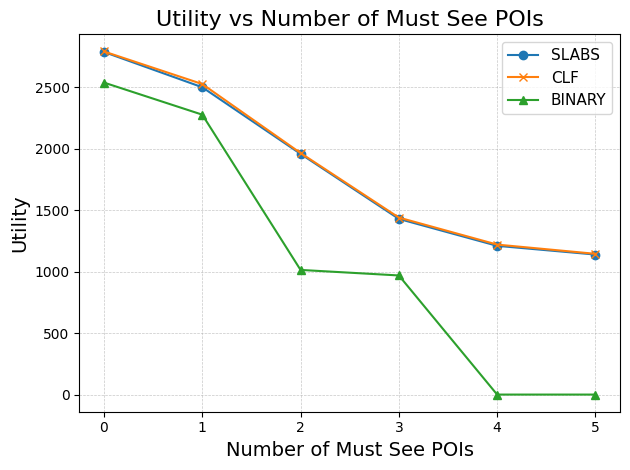
\includegraphics[width=0.48\columnwidth]{plots/mustsee.png}
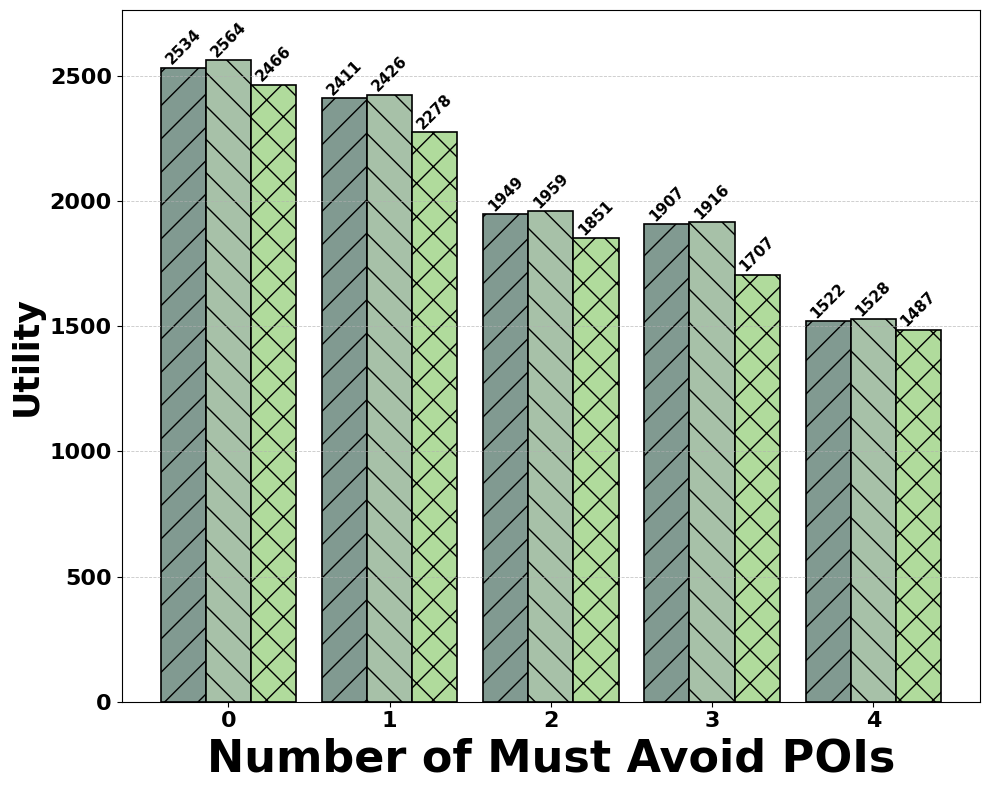
\includegraphics[width=0.48\columnwidth]{plots/mustavoid.png}
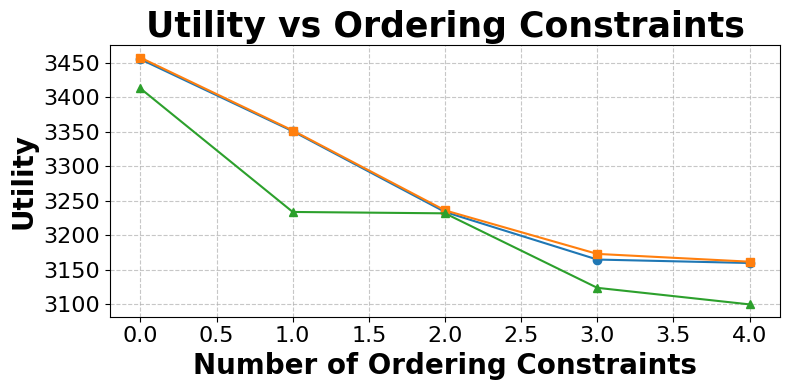
\includegraphics[width=0.48\columnwidth]{plots/ordering.png}
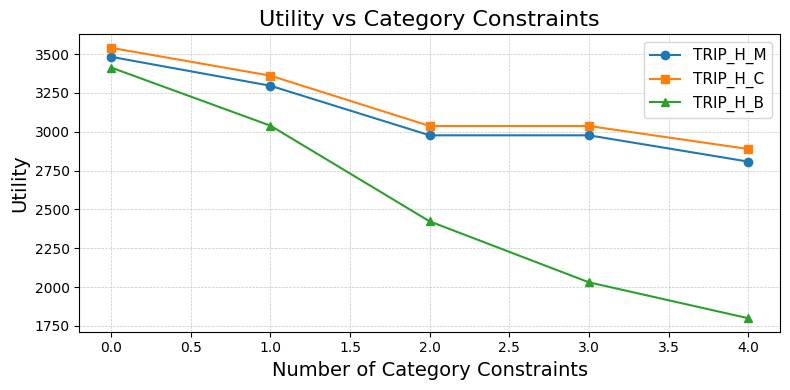
\includegraphics[width=0.48\columnwidth]{plots/category.png}
\figcaption{Various personalized constraints}
\label{fig:personalizedconstraints}
\end{figure}

Fig.~\ref{fig:personalizedconstraints} shows the results of various personalized constraints over the 3 utility variants.
In this study, a cost budget of 6000 units and a time budget of 480 minutes is fixed across all the cases.
With multiple must-see POIs fixed by the traveler, the utility falls, since there is not much scope for the solver to optimize. The same happens with multiple must-avoid POIs, although the decline is less sharp.
The same reduction in utility is observed with more number of ordering and category constraints.
Binary shows the sharpest drops since it has the least leeway; Slab and Continuous variants can partially visit a POI, and move to other POIs for better utility gain.

\subsection{Dynamic Re-planning}

\begin{figure}[th]
    \centering
    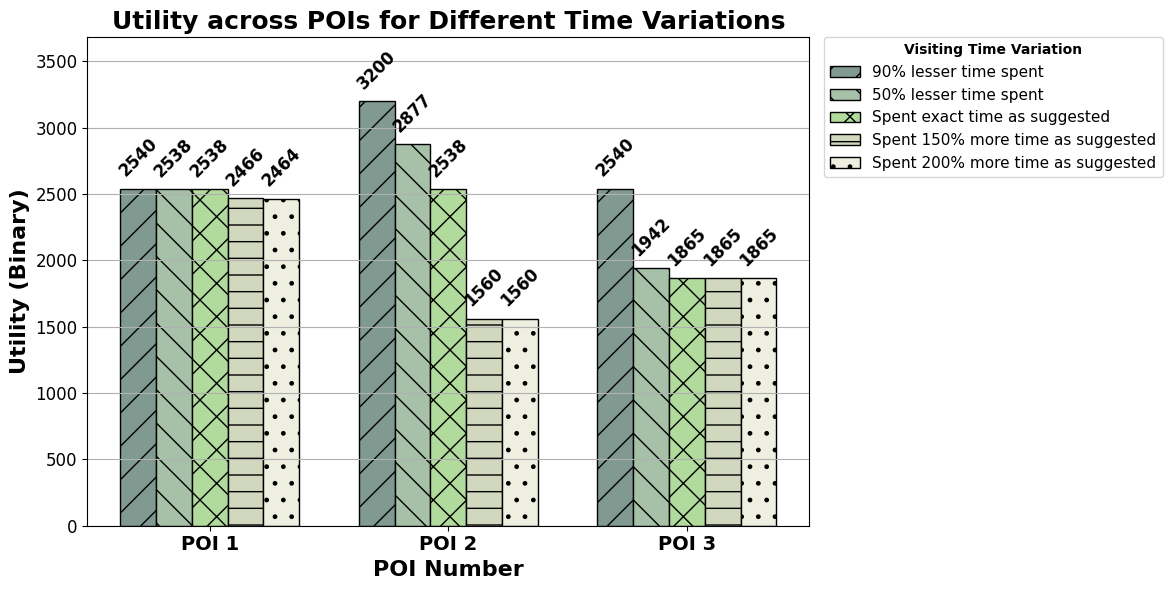
\includegraphics[width=\figwidth]{plots/dynamic_pkj.png}
    \figcaption{Dynamic re-planning after tourist spends less or more time at a POI}
    \label{fig:dynamic}
\end{figure}

The next experiment captures the changes in utility when dynamic re-planning is done.
Fig.~\ref{fig:dynamic} covers five different scenarios for a POI, according to the time spent in visiting it: (1)~\emph{50\% less}, i.e., when the traveler spends 50\% of the visit time prescribed, (2)~\emph{25\% less}, i.e., 75\% of the prescribed time, (3)~\emph{ontime}, i.e., when the traveler spends the exact prescribed time, (4)~\emph{50\% more}, i.e., 150\% of the prescribed time, and (5)~\emph{100\% more}, i.e., 200\% of the prescribed time.
The different groups specify the \emph{order} of the POI where the change is made (all other POIs spent the exact prescribed time).
In order to take the readings for the plot, we modified the average visit time of the POIs of Osaka so as to bring more clarity in the result, which made the trends observed in the case of the variable time spent by the user on the POI.
This was done only for this experiment.
The time and cost budget are 480 minutes and 6000 units respectively.
The optimal static itinerary consists of 4 POIs.
Our planner dynamically recalculates the itinerary by considering the actual time a user spends at each Point of Interest (POI) and the time taken to travel between them, in contrast to the initially suggested schedule.

The figure shows that the effect of spending a substantially different time on the first POI does not have much effect, since there is enough time for the planner to find another itinerary with a similar utility.
Similarly, spending less time in the third POI does not give a much better itinerary since there is not much scope to maneuver, given the time budget already spent. Spending a lot of extra time may, however, decrease the utility significantly, especially if this does not allow reaching the fourth and subsequent POIs.
The most amount of variability is visible for the second POI.
Spending lesser times results in re-planning significantly better itineraries, while spending much longer times results in lesser utility itineraries, despite re-planning.

Overall, this variation in utility values underscores the importance of adapting the itinerary based on real-time user behavior, demonstrating the effectiveness of our dynamically responsive planning approach.

\subsection{Scalability}

In this section, we test the scalability of our MILP solution in terms of running time for various parameters.

Fig.~\ref{fig:number-of-pois} and Fig.~\ref{fig:number-of-days} show that the time increases exponentially with number of POIs and number of days in the trip, which is expected for a linear programming solution.
Importantly, the computation times remain \emph{practical} even when the number of POIs or the number of days is very high.

\begin{figure}[t]
    \centering
    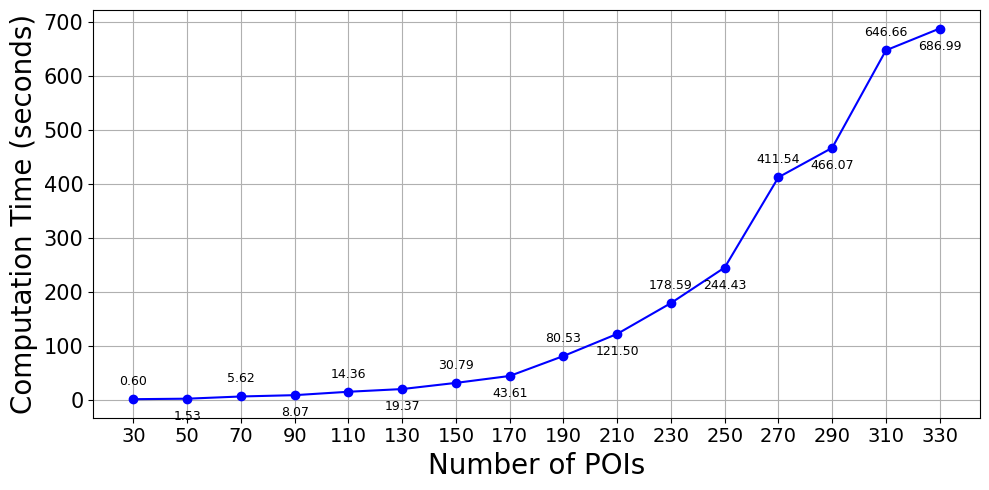
\includegraphics[width=\figwidth]{plots/scalability_new_pkj.png}
    \figcaption{Scalability with number of POIs}
    \label{fig:number-of-pois}
\end{figure}

\begin{figure}[t]
    \centering
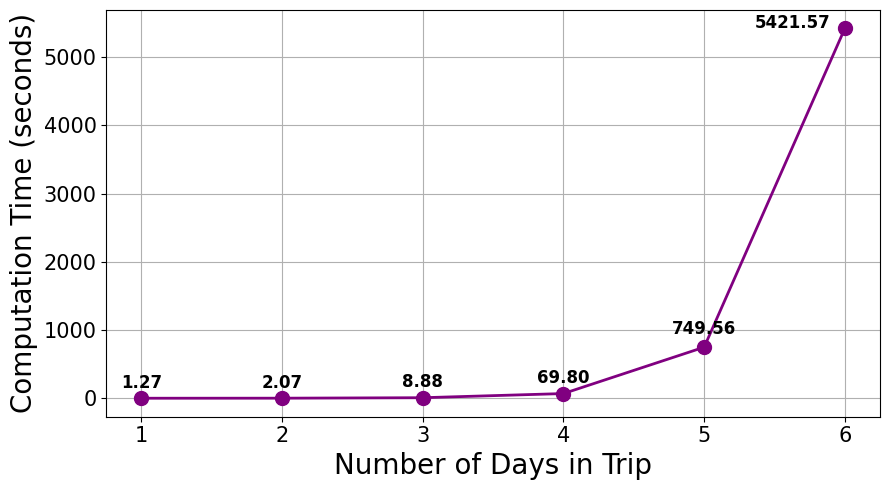
\includegraphics[width=\figwidth]{plots/scalability_multiday.png}
     \figcaption{Scalability with number of days in multi-day trips}
    \label{fig:number-of-days}
\end{figure}

We next show the change in computation time when the cost and time budget change.
As shown in Fig.~\ref{fig:cost-budget}, for extremely low cost budgets, the time taken is small, but it increases rapidly with increasing cost budget. This is due to the fact that more choices become available when the cost budget increases. However, once the cost budget exceeds a threshold, the solver can effectively ignore about it, since almost all solutions become feasible in terms of cost.
Similarly, the computation time remains very low, unless the time budget is extremely high (Fig.~\ref{fig:time-budget}) since only then almost all solutions become feasible in terms of time.

\begin{figure}[t]
    \centering
    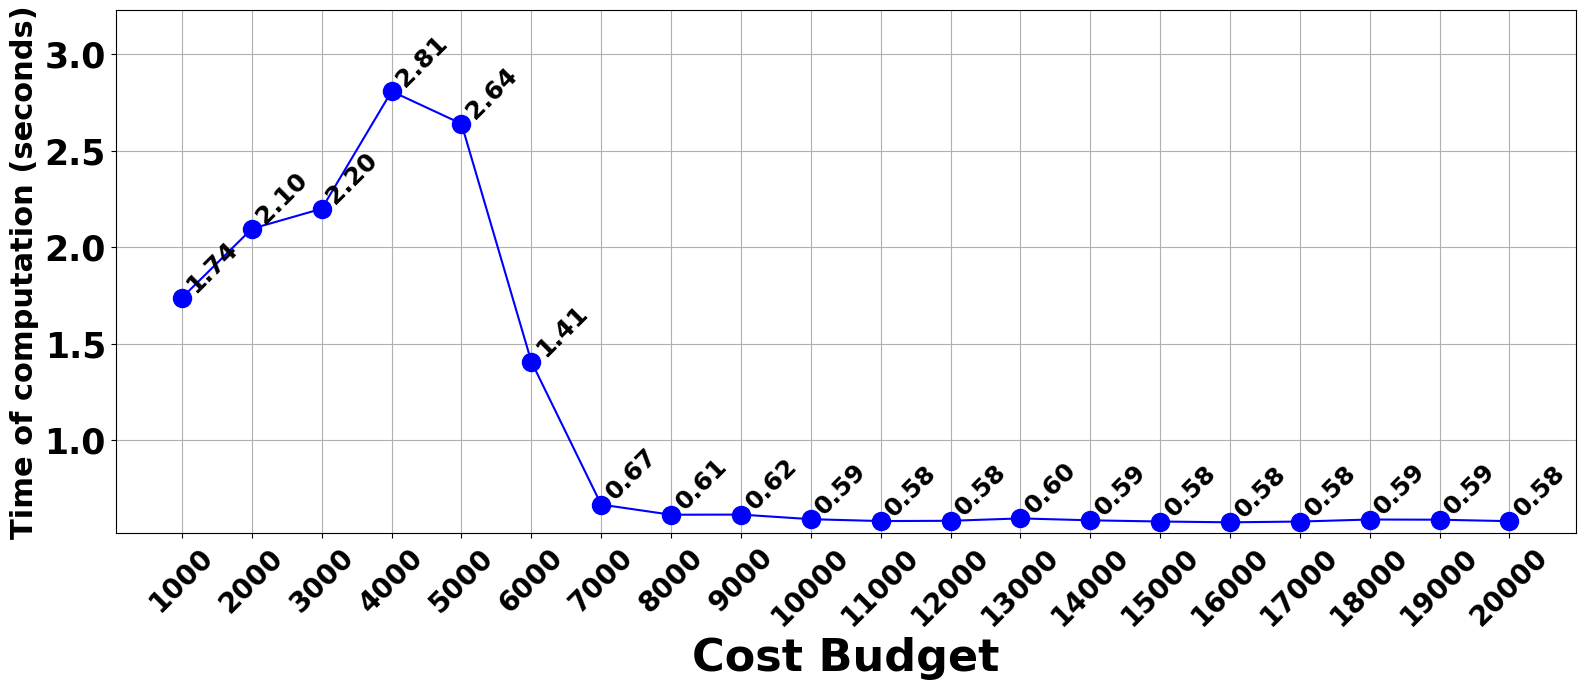
\includegraphics[width=\figwidth]{plots/costbudgetvstoc.png}
    \figcaption{Time of computation on increasing cost budget at fixed time budget 480 minutes}
    \label{fig:cost-budget}
\end{figure}

\begin{figure}[t]
    \centering
    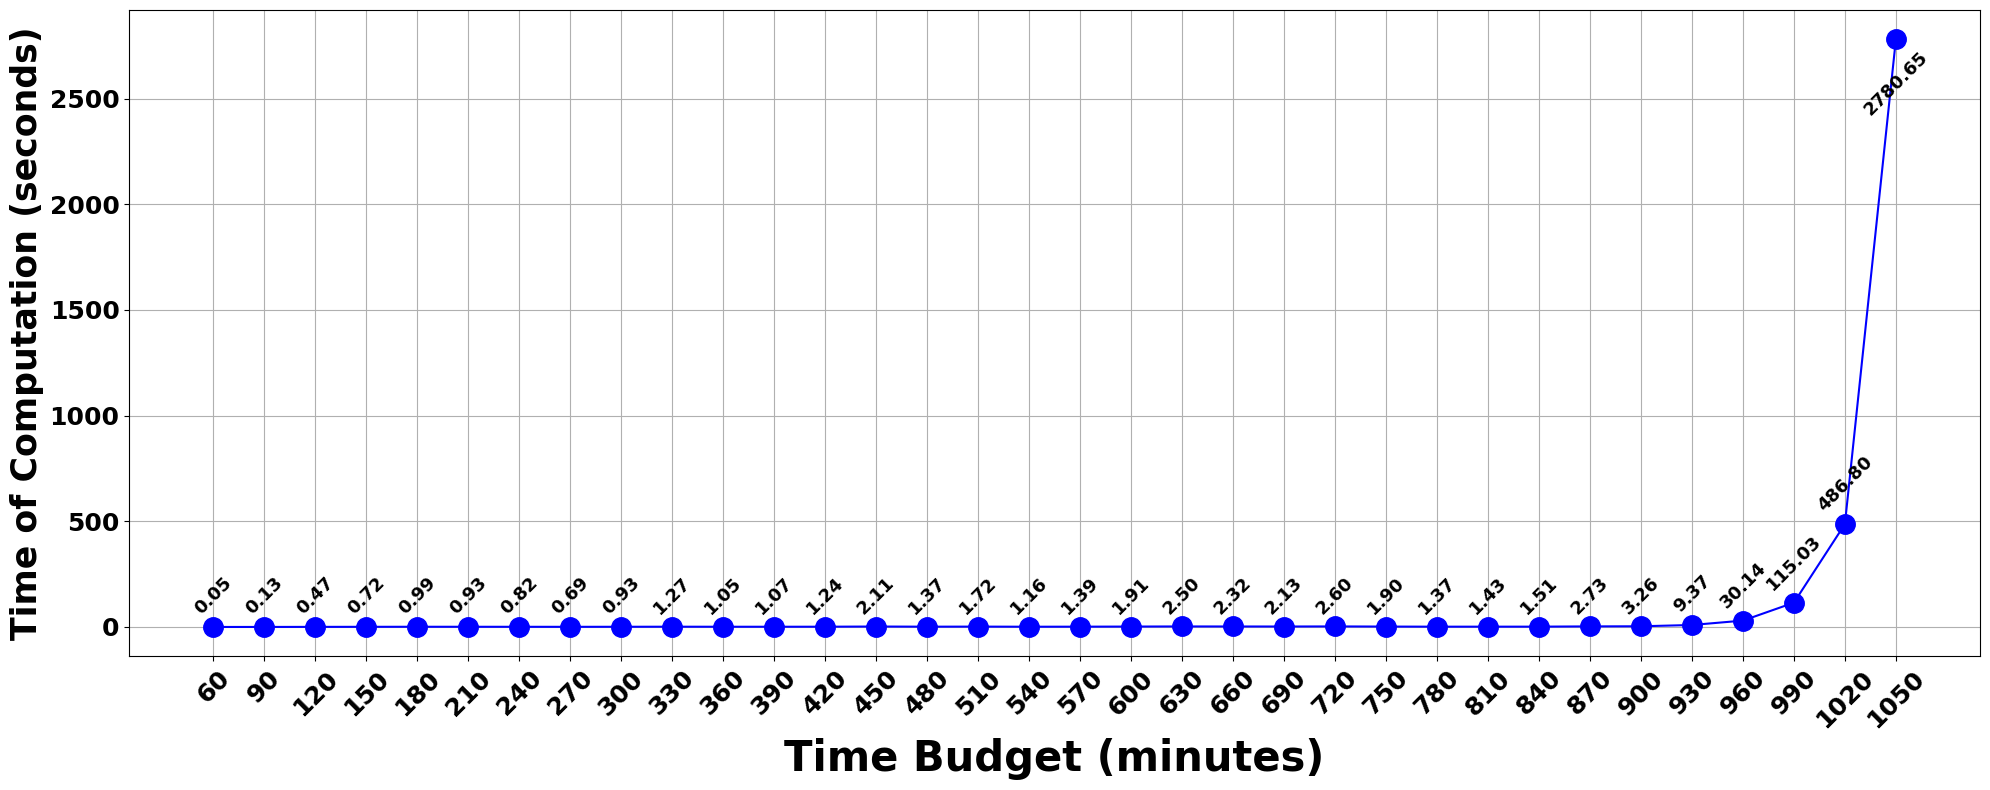
\includegraphics[width=\figwidth]{plots/timebudgetvstoc.png}
    \figcaption{Time of computation on increasing time budget at fixed cost budget 6000 units}
    \label{fig:time-budget}
\end{figure}

\subsection{Summary of Experimental Results}

Overall, our experimental results provide the following insights.
The \trip variants outperform the baseline significantly.
The Hybrid is the best mode of transport.
The Continuous utility variant gives slightly better results than the Slab variant, and both of them outperform the Binary variant due to lack of flexibility for the Binary variant.
Optimizing for multiple days in one shot gives significantly better results than solving for single days, and adding them up.
Personalized constraints are handled efficiently by our \trip solution.
Dynamic re-planning can increase the utility when there is scope to maneuver the rest of the plan.
Finally, \trip solver, despite being a MILP solution, is practical.

